\newcommand{\ClassPath}{../VIU_TFM_LaTeX_template}
\documentclass{\ClassPath/viu-tfm-template}
\usepackage{multicol}

\definecolor{maincolor}{HTML}{f25416}

%--------------------------------------------------------------------------
% Definiciones necesarias Modifica con tus datos
%--------------------------------------------------------------------------
\def\nombre{Gómez Olivencia, Rubén}
\def\dni{78910013-A}
\def\titulo{Evolución de las tareas en un proyecto Web\linebreak\linebreak(Scrum daily meetings)}
\def\subtitulo{}
\def\titulacion{Máster Universitario en Desarrollo de Aplicaciones y Servicios Web}
\def\curso{2022-2023}

%Los siguientes son opcionales: si no se ponen, la portada cambia un poco. Ideal para escribir artículos/trabajos cortos
\def\dirige{}
\def\codirige{}
\def\convocatoria{}
\def\asignatura{Gestión de proyectos en entornos ágiles}


% importar fichero de Bibliografía
%\addbibresource{Actividad_1.bib}

\begin{document}
    \graphicspath{{../VIU_TFM_LaTeX_template/}}

    \coverpage

    \tableofcontents

\chapter{Introducción}

A la hora de gestionar un proyecto es conveniente hacer uso de las tecnologías ágiles que están de moda, pero eso no supone sólo realizar un análisis previo.

Durante la vida del proyecto hay que ir tomando decisiones teniendo en cuenta el estado del proyecto, de las tareas realizadas (y a realizar) y cuál es el estado del equipo que lo desarrolla. Con todo esto, y con otras posibles variables externas, habrá que ir adaptando la gestión del proyecto para buscar la manera más eficiente de continuar con el desarrollo.

A lo largo de este documento se van a realizar dos simulaciones de la gestión de un proyecto web, en las que se plasmarán todos los pasos realizados, así como el tiempo que ha llevado el terminar el proyecto para cada una de ellas.


\chapter{Requisitos del proyecto}

Para la simulación del proyecto se va a tener en cuenta que el equipo de desarrollo va a constar de cuatro personas:

\begin{itemize}
    \item John
    \item Susan
    \item Robert
    \item Emily
\end{itemize}

Los cuatro desarrolladores tienen un perfil que se puede considerar multidisciplinar, y que por tanto son capaces de realizar cualquier tarea dentro del proyecto.

En lo que a tareas se refiere, el proyecto va a contar con una serie de tareas en las que se va a indicar:
\begin{itemize}
    \item El \textbf{nombre} de la tarea, que determina, a grandes rasgos, lo que se debe realizar.
    \item El \textbf{coste} en horas del tiempo estimado para la realización de la tarea.
    \item El límite inicial establecido (en días) para terminar la tarea.
\end{itemize}

\begin{columntblr}{XXX}
    Tareas de programación & Coste & Límite inicial
    establecido (días) \\
    Login & 20 & 6 \\
    API Rest & 20 & 6 \\
    Integrar MongoDB & 17 & 2 \\
    Crear Foro & 19 & 3 \\
    UI & 25 & 4 \\
    Chat & 24 & 4 \\
    Analytics & 7 & 4 \\
\end{columntblr}

Teniendo en cuenta estas tareas, pasaremos a realizar las simulaciones.

\chapter{Simulaciones de la gestión del proyecto}

A continuación se van a detallar cómo se han realizado las simulaciones, lo acontecido en las reuniones diarias de Scrum y las decisiones tomadas para el avance del proyecto.

Para ambas simulaciones el panel Kanban inicial va a tener el siguiente aspecto:

\begin{center}
    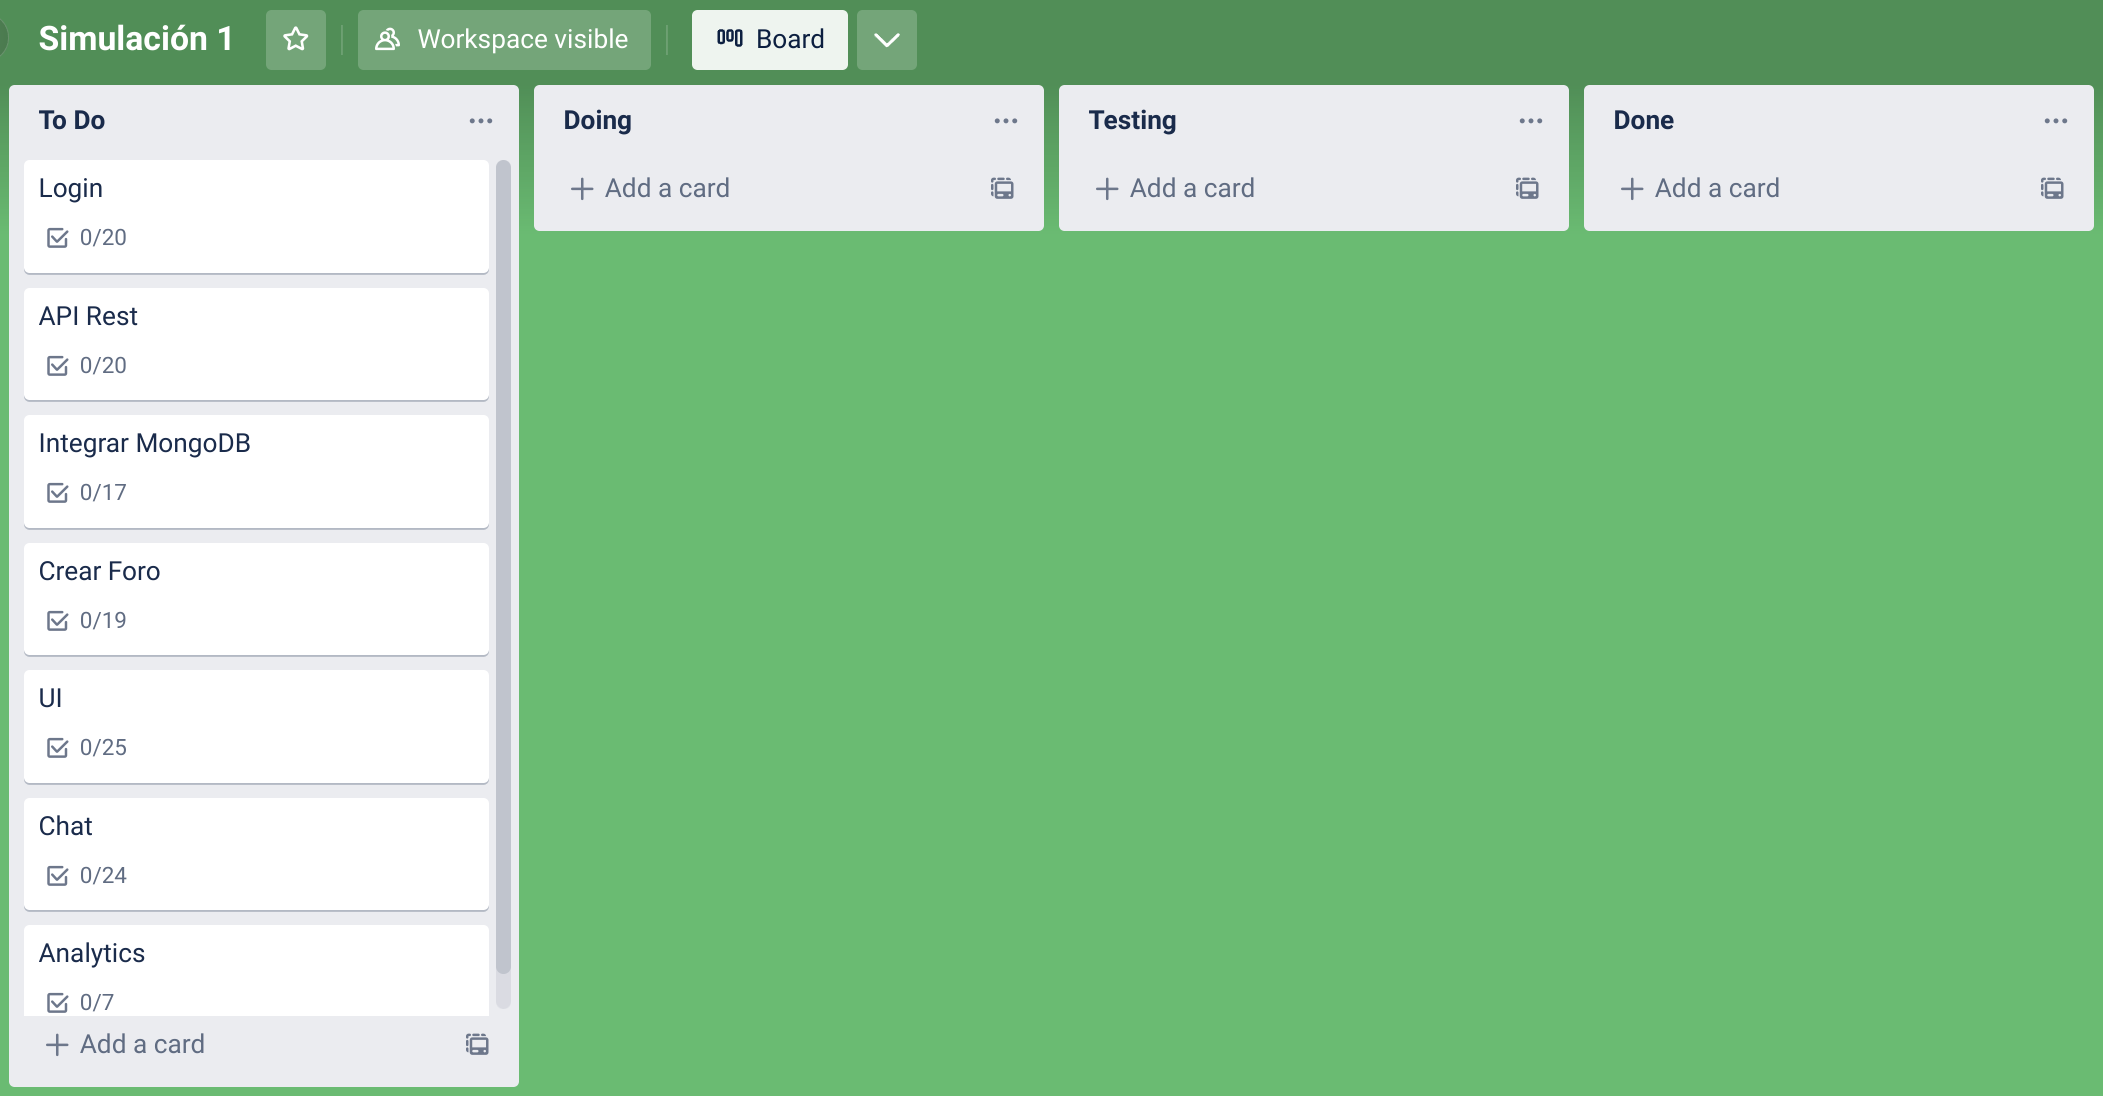
\includegraphics[width=0.93\linewidth]{img/general.png}
\end{center}

En cada tarea se ha añadido un “contador de horas” que corresponde con la estimación inicial (en Trello hecho a través de un “\textit{checklist}”). De esta manera visualmente es sencillo visualizar el estado de cada tarea.

Para la asignación de tareas se van a utilizar etiquetas de distintos colores, y así también se podrá filtrar por desarrollador. Para simular el avance diario realizado para cada tarea se utilizará un dado de seis caras (que indicará el número de horas reales avanzadas en la tarea).

\section{Simulación 1}

En la primera simulación en las “\textit{daily meeting}” de Scrum entre todos los miembros se decidirá cómo repartir las tareas y el tiempo (en días) que estará cada persona con la tarea correspondiente.

\subsection{Reunión 1}
En la primera reunión se decide el reparto inicial de tareas. Para la tarea “Integar MongoDB”, dado que hay pocos días para hacerla, se le asignan dos personas.

\begin{columntblr}{XX[2]XXX}
    Reunión 1 & Tarea actual & Avance diario & Estado final/día & Días usados\\
    John & Login & 6 & 6/20 & 1/6\\
    Susan & API Rest & 5 & 5/20 & 1/6\\
    Robert & Integrar MongoDB & 2 & 6/17 & 1/2\\
    Emily & Integrar MongoDB & 4 & 6/17 & 1/2\\
\end{columntblr}

\begin{center}
    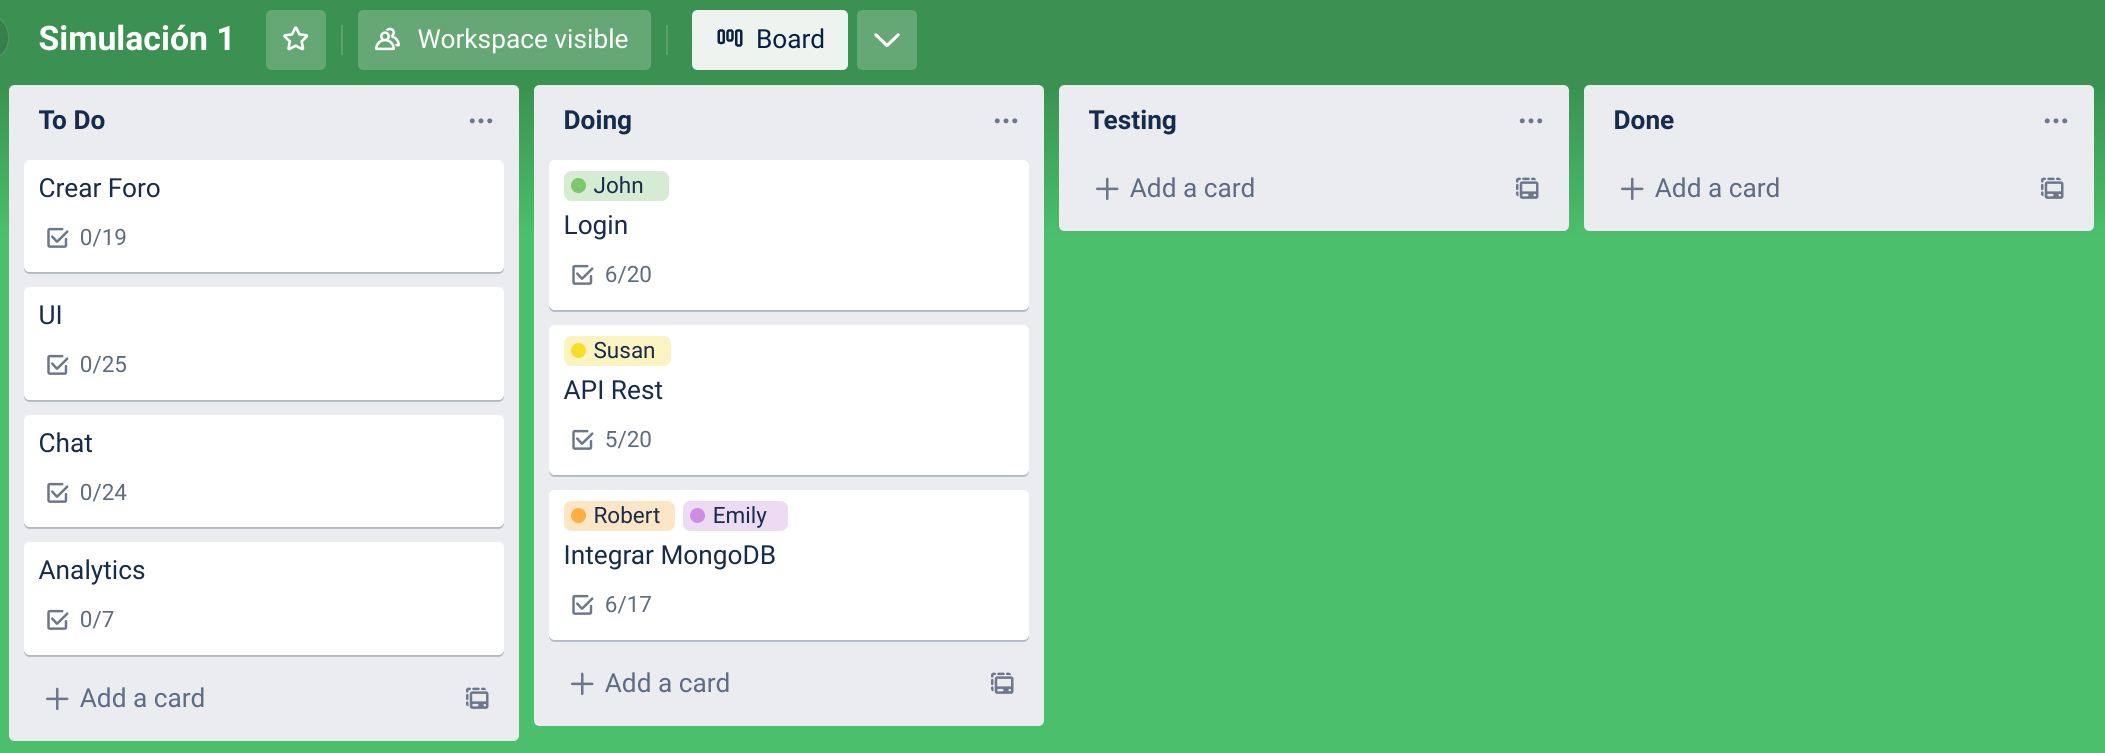
\includegraphics[width=\linewidth]{img/s1-1.png}
\end{center}

Tras terminar el día, tal como se puede ver en la tabla y en la imagen de Trello, ha habido cierto avance para algunas de las tareas.

\subsection{Reunión 2}
Tras el primer día, se analiza el estado de las tareas y ya se comprueba cómo la tarea “Integrar MongoDB” es bastante probable que no pueda ser terminada a lo largo del día de hoy. Hay que esperar, pero la estimación parece haber sido demasiado positiva.

\begin{columntblr}{XX[2]XXX}
    Reunión 2 & Tarea actual & Avance diario & Estado final/día & Días usados\\
    John & Login & 1 & 7/20 & 2/6\\
    Susan & API Rest & 4 & 9/20 & 2/6\\
    Robert & Integrar MongoDB & 6 & 16/17 & 2/2\\
    Emily & Integrar MongoDB & 4 & 16/17 & 2/2\\
\end{columntblr}

\begin{center}
    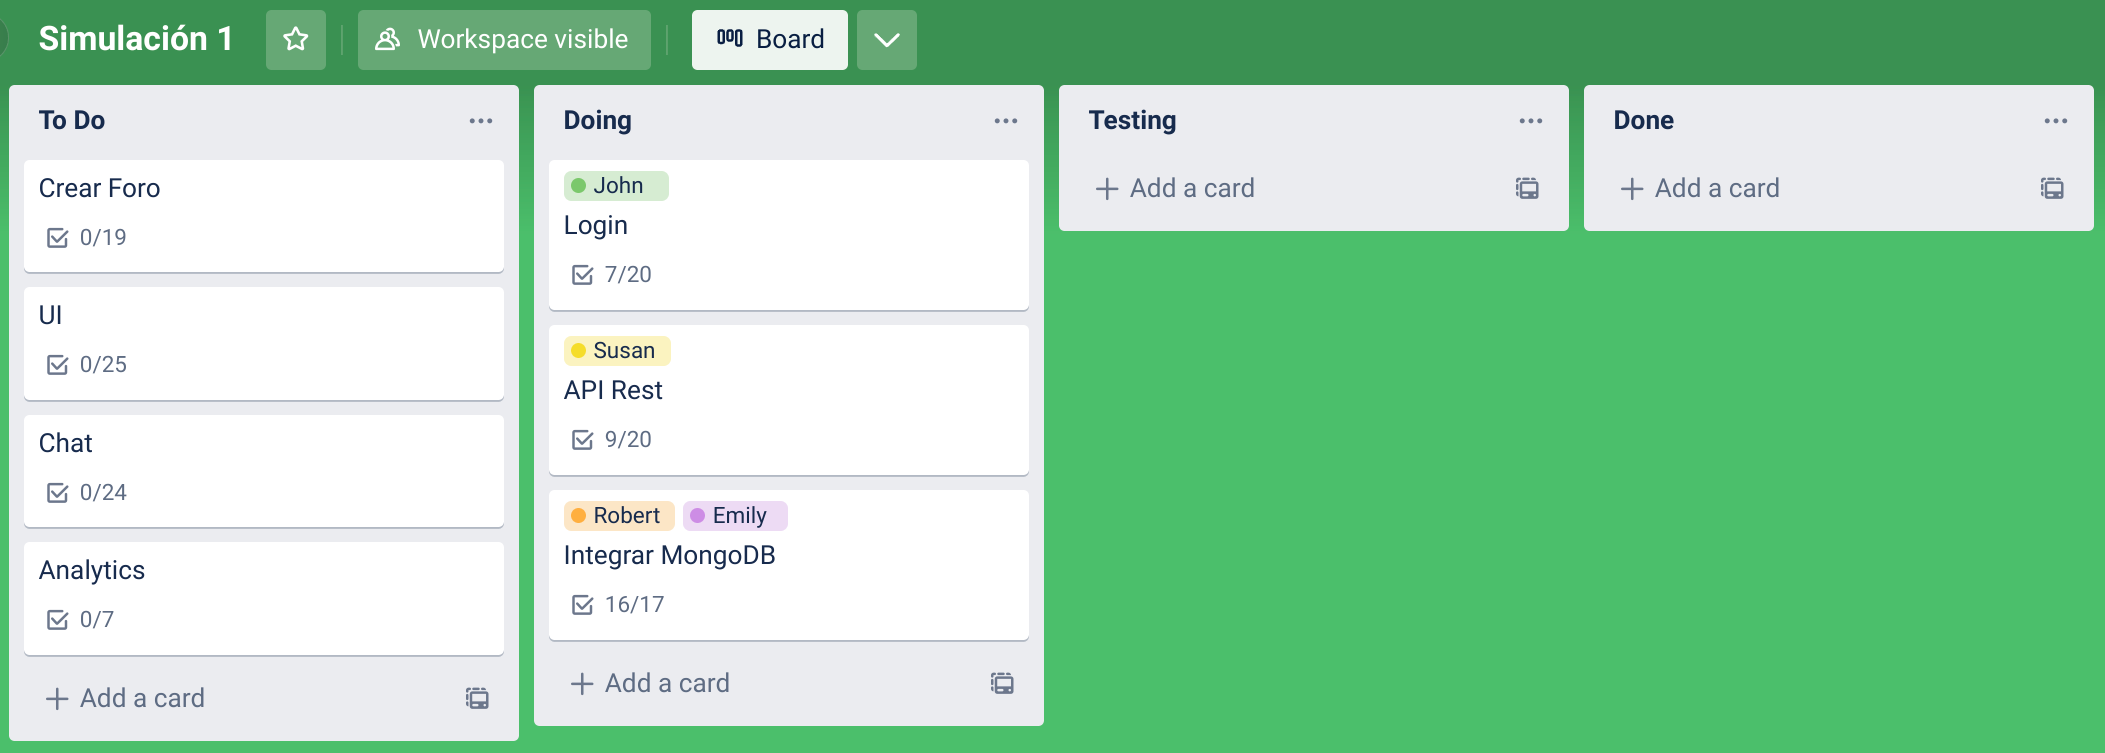
\includegraphics[width=\linewidth]{img/s1-2.png}
\end{center}

\subsection{Reunión 3}
Tal como se comentó en el día anterior, la tarea “Integrar MongoDB” no ha sido finalizada a tiempo, pero por poco. Se decide dejar sólo a Robert con la tarea y se estima que el día de hoy se va a terminar. Emily pasa a la siguiente tarea.

Ahora bien, si Robert consigue terminar la tarea hoy, se unirá a Emily en la tarea “Crear Foro”.

\begin{columntblr}{XX[2]XXX}
    Reunión 3 & Tarea actual & Avance diario & Estado final/día & Días usados\\
    John & Login & 3 & 10/20 & 3/6\\
    Susan & API Rest & 5 & 14/20 & 3/6\\
    Robert & Integrar MongoDB & 1 & 17/17 & 3/2\\
    Emily & Crear Foro & 6 & 10/19 & 1/3\\
    Robert & Crear Foro & 4 & 10/19 & 1/3\\
\end{columntblr}

Tal como se puede ver, Robert ha conseguido terminar la tarea y se ha unido a Emily en la tarea “Crear Foro”.

\begin{center}
    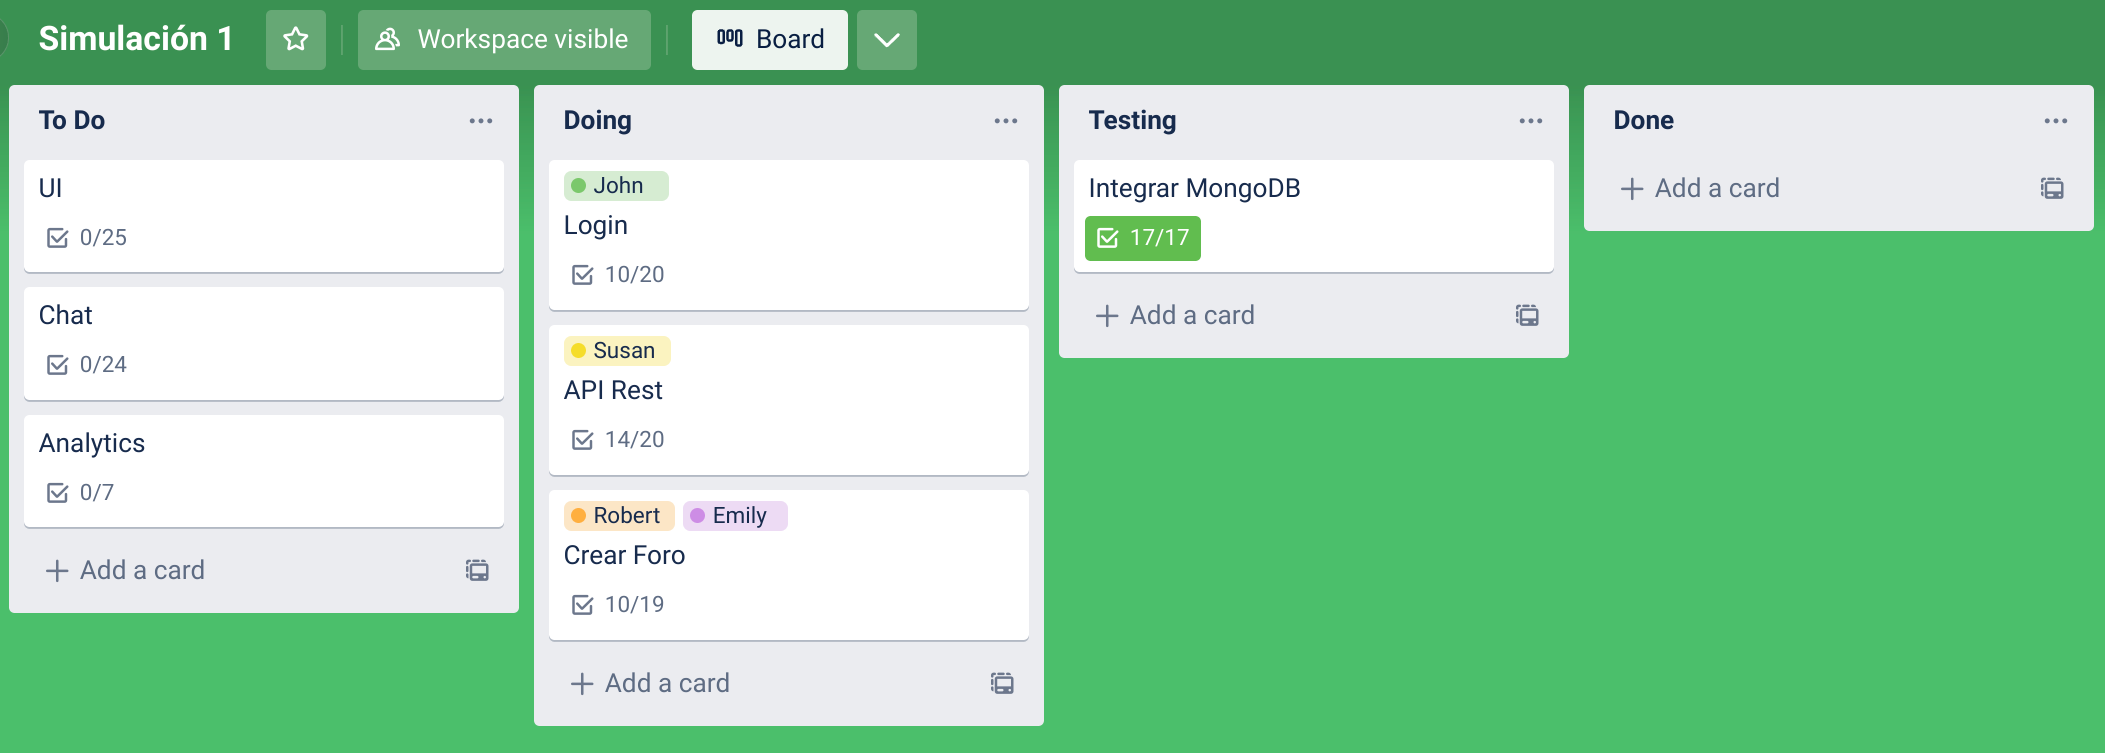
\includegraphics[width=\linewidth]{img/s1-3.png}
\end{center}

\subsection{Reunión 4}
Ayer se consiguió terminar “Integrar MongoDB” y dado que no ha habido ningún cambio en el resto, se mantienen las asignaciones:

\begin{columntblr}{XX[2]XXX}
    Reunión 4 & Tarea actual & Avance diario & Estado final/día & Días usados\\
    John & Login & 4 & 14/20 & 4/6\\
    Susan & API Rest & 4 & 18/20 & 4/6\\
    Emily & Crear Foro & 5 & 16/19 & 2/3\\
    Robert & Crear Foro & 1 & 16/19 & 2/3\\
\end{columntblr}

Trello al terminar el día queda:
\begin{center}
    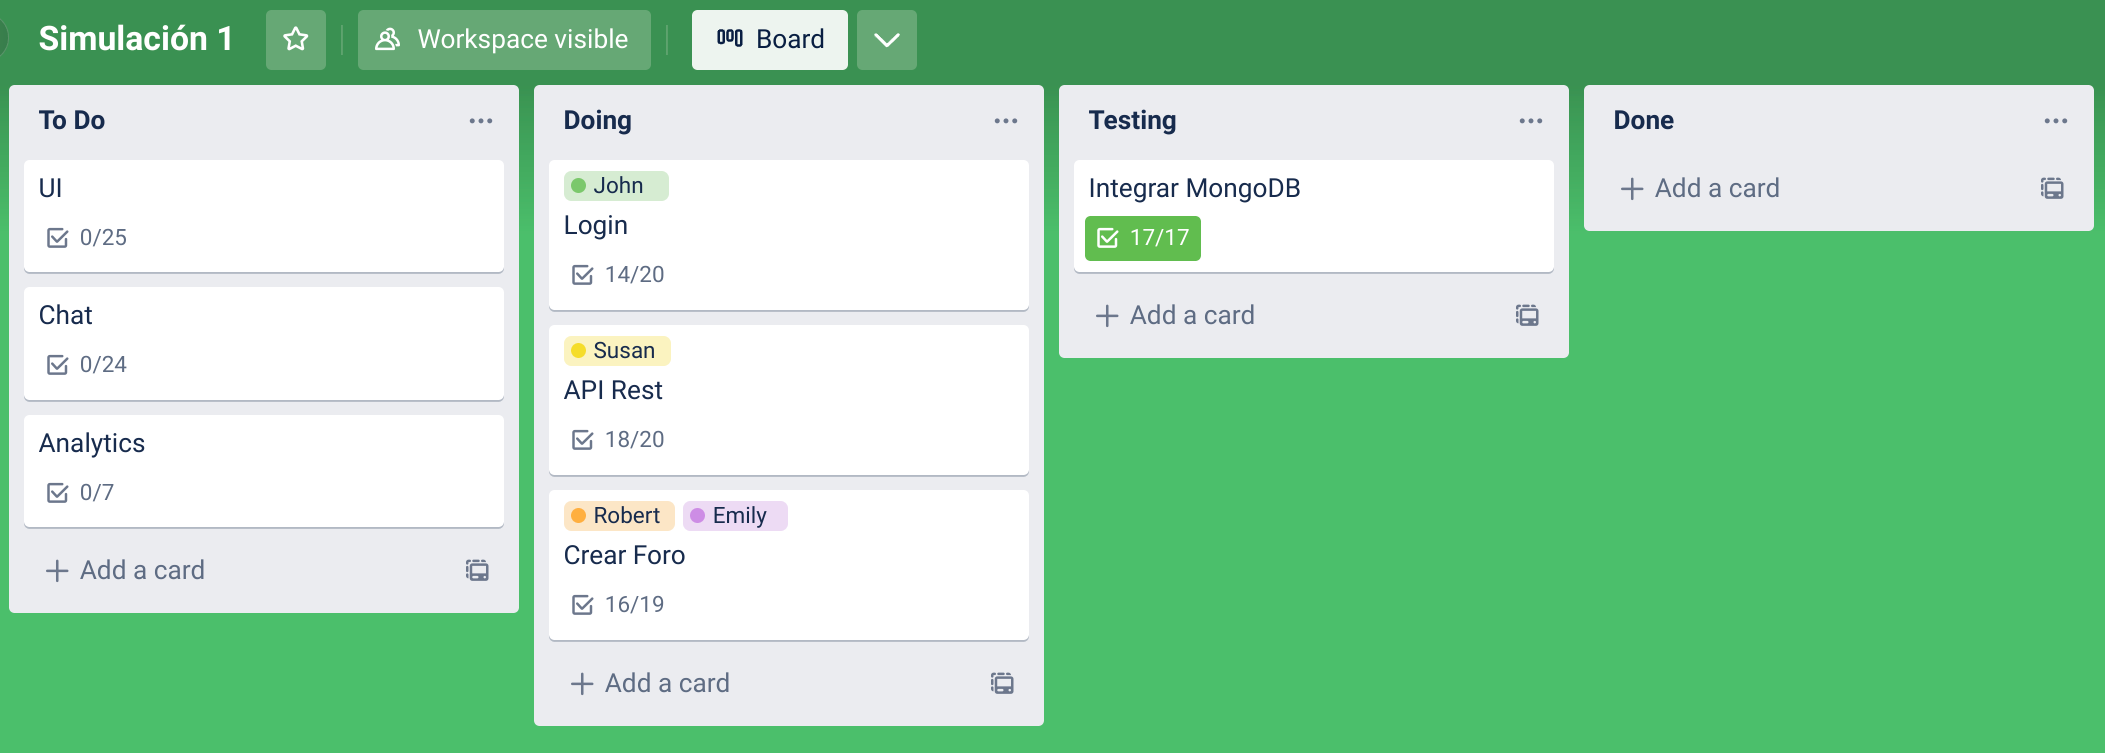
\includegraphics[width=\linewidth]{img/s1-4.png}
\end{center}

\subsection{Reunión 5}
Teniendo en cuenta los avances del día anterior, se decide que si Susan termina hoy la tarea, trate de ponerse con “UI”. En el caso de Emily y Robert, lo mismo para la tarea “Chat”, ya que su estimación de días es muy ajustada.

\begin{columntblr}{XX[2]XXX}
    Reunión 5 & Tarea actual & Avance diario & Estado final/día & Días usados\\
    John & Login & 5 & 19/20 & 5/6\\
    Susan & API Rest & 1 & 19/20 & 5/6\\
    Emily & Crear Foro & 1 & 19/19 & 3/3\\
    Robert & Crear Foro & 2 & 19/19 & 3/3\\
    Robert & Chat & 2 & 2/24 & 1/4\\
\end{columntblr}

Al finalizar el día el Trello queda de la siguiente manera:
\begin{center}
    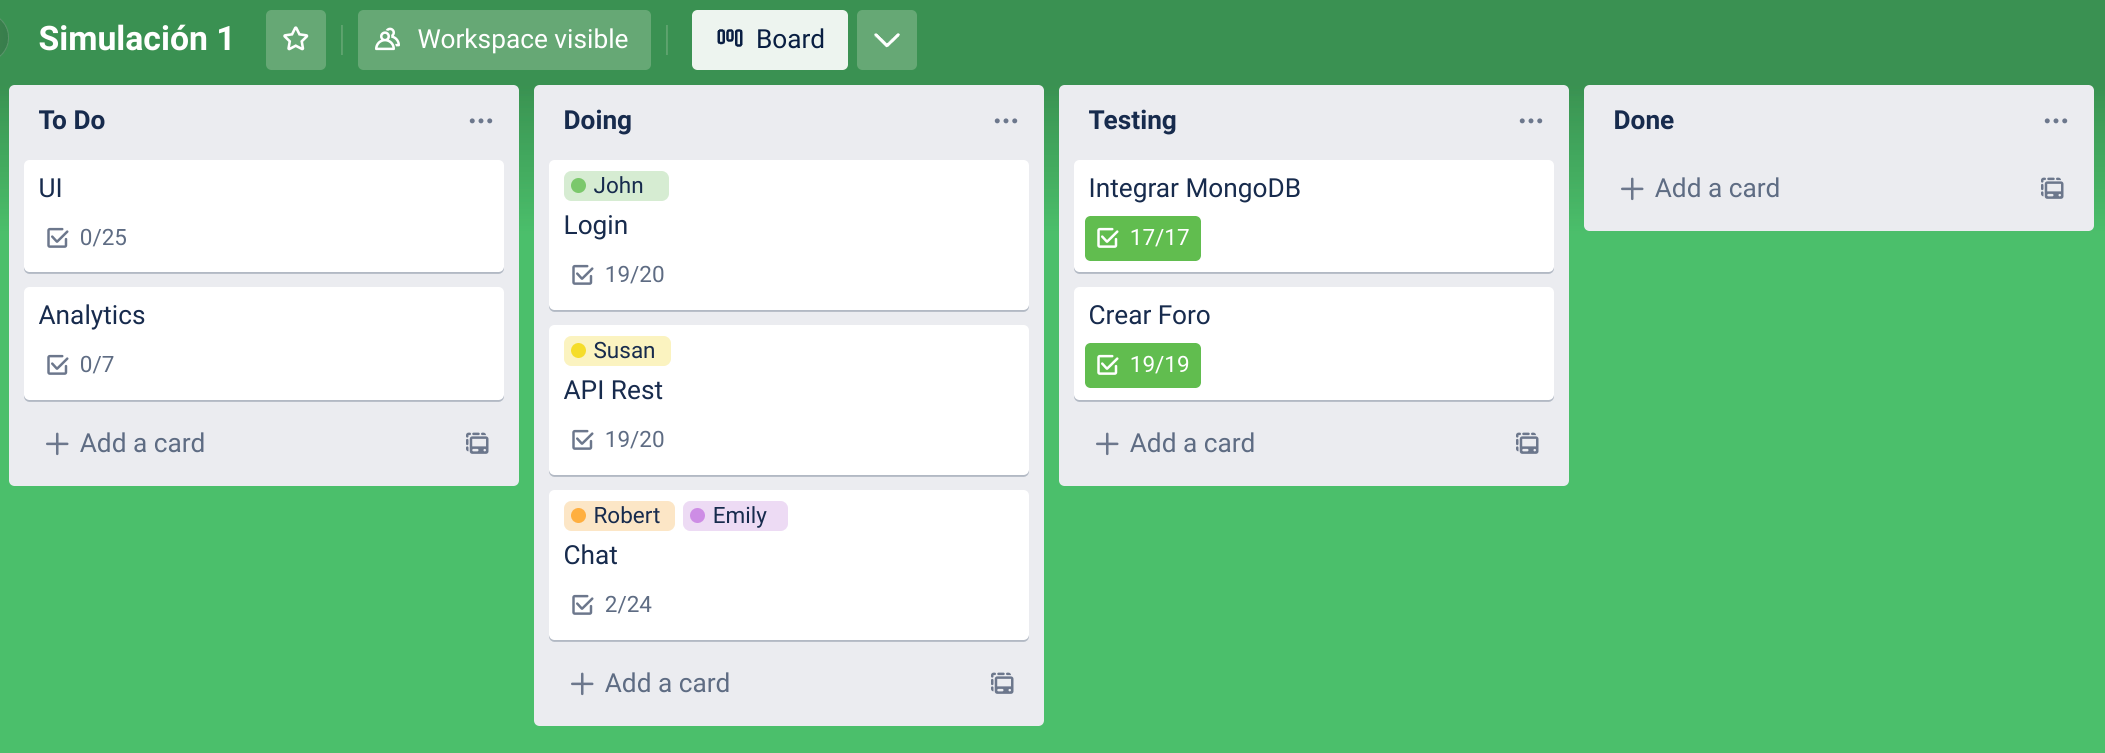
\includegraphics[width=\linewidth]{img/s1-5.png}
\end{center}

\subsection{Reunión 6}
Tal como se quedaron las tareas el día anterior, se decide cambiar la previsión para el día de hoy. Como todo apunta a que John y Susan terminarán sus tareas, en cuanto terminen ambos se pondrán con “UI”. Robert y Emily seguirán avanzando con “Chat”.

\begin{columntblr}{XX[2]XXX}
    Reunión 6 & Tarea actual & Avance diario & Estado final/día & Días usados\\
    John & Login & 1 & 20/20 & 6/6\\
    Susan & API Rest & 1 & 20/20 & 6/6\\
    Emily & Chat & 1 & 4/24 & 2/4\\
    Robert & Chat & 1 & 4/24 & 2/4\\
    John & UI & 2 & 2/25 & 1/5\\
\end{columntblr}


\begin{center}
    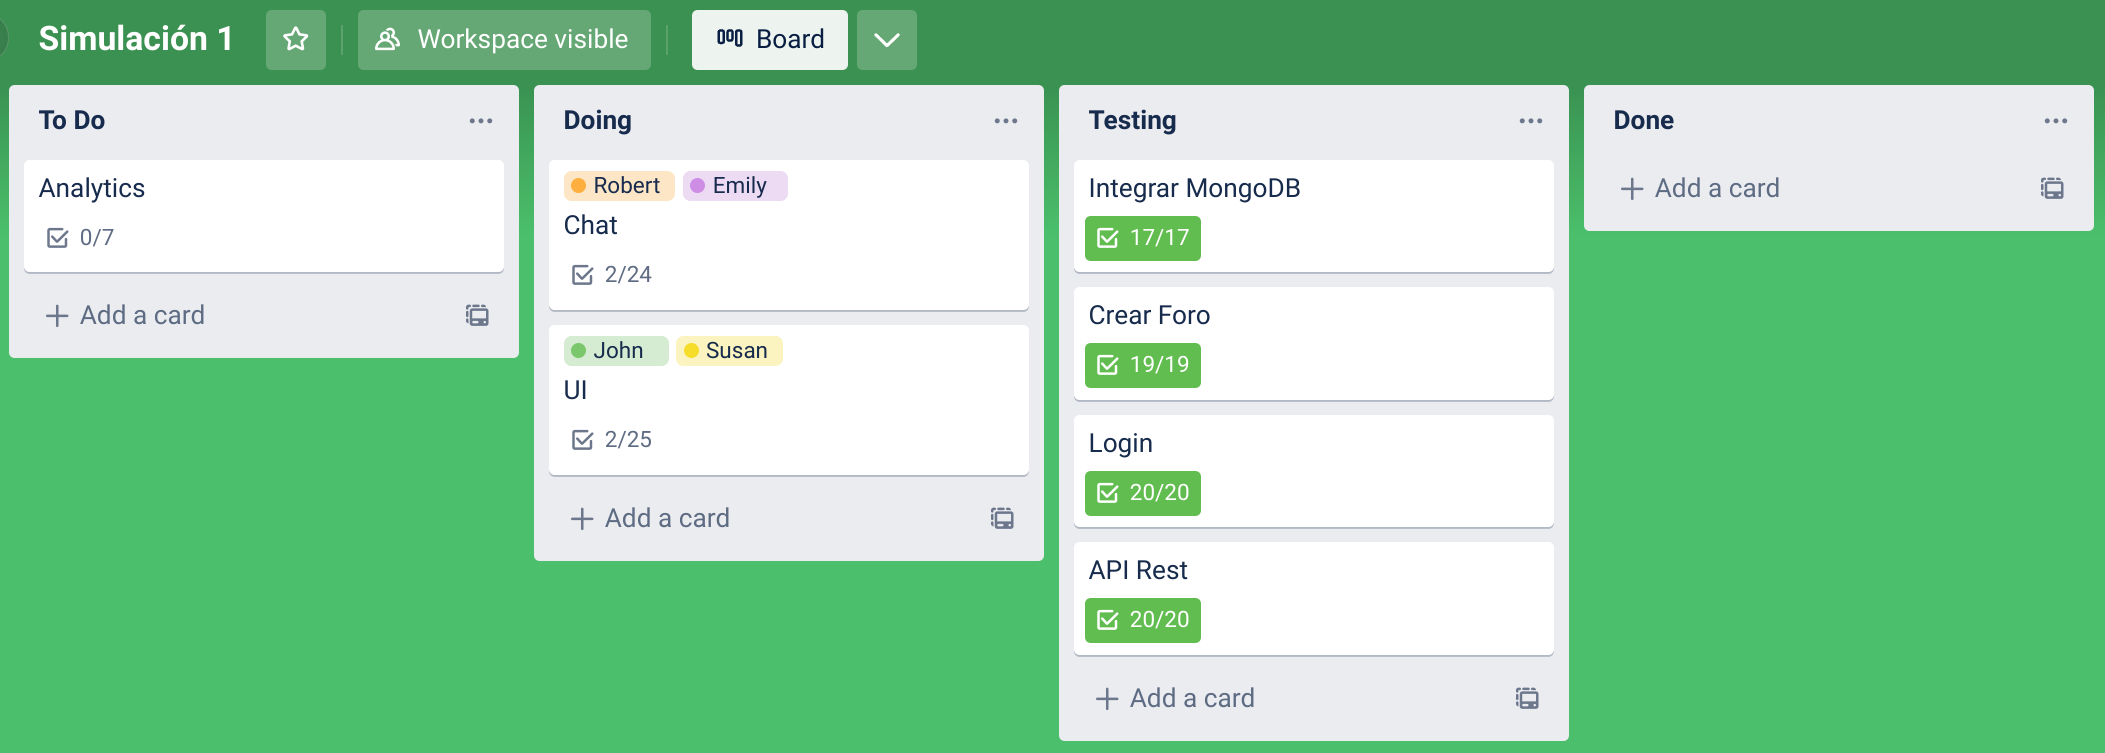
\includegraphics[width=\linewidth]{img/s1-6.png}
\end{center}

\subsection{Reunión 7}
Ayer no se avanzó demasiado, por lo que durante el día de hoy se mantienen las asignaciones.

\begin{columntblr}[long]{XX[2]XXX}
    Reunión 7 & Tarea actual & Avance diario & Estado final/día & Días usados\\
    John & UI & 4 & 9/25 & 2/5\\
    Susan & UI & 3 & 9/25 & 2/5\\
    Emily & Chat & 4 & 9/24 & 3/4\\
    Robert & Chat & 1 & 9/24 & 3/4\\
\end{columntblr}

\begin{center}
    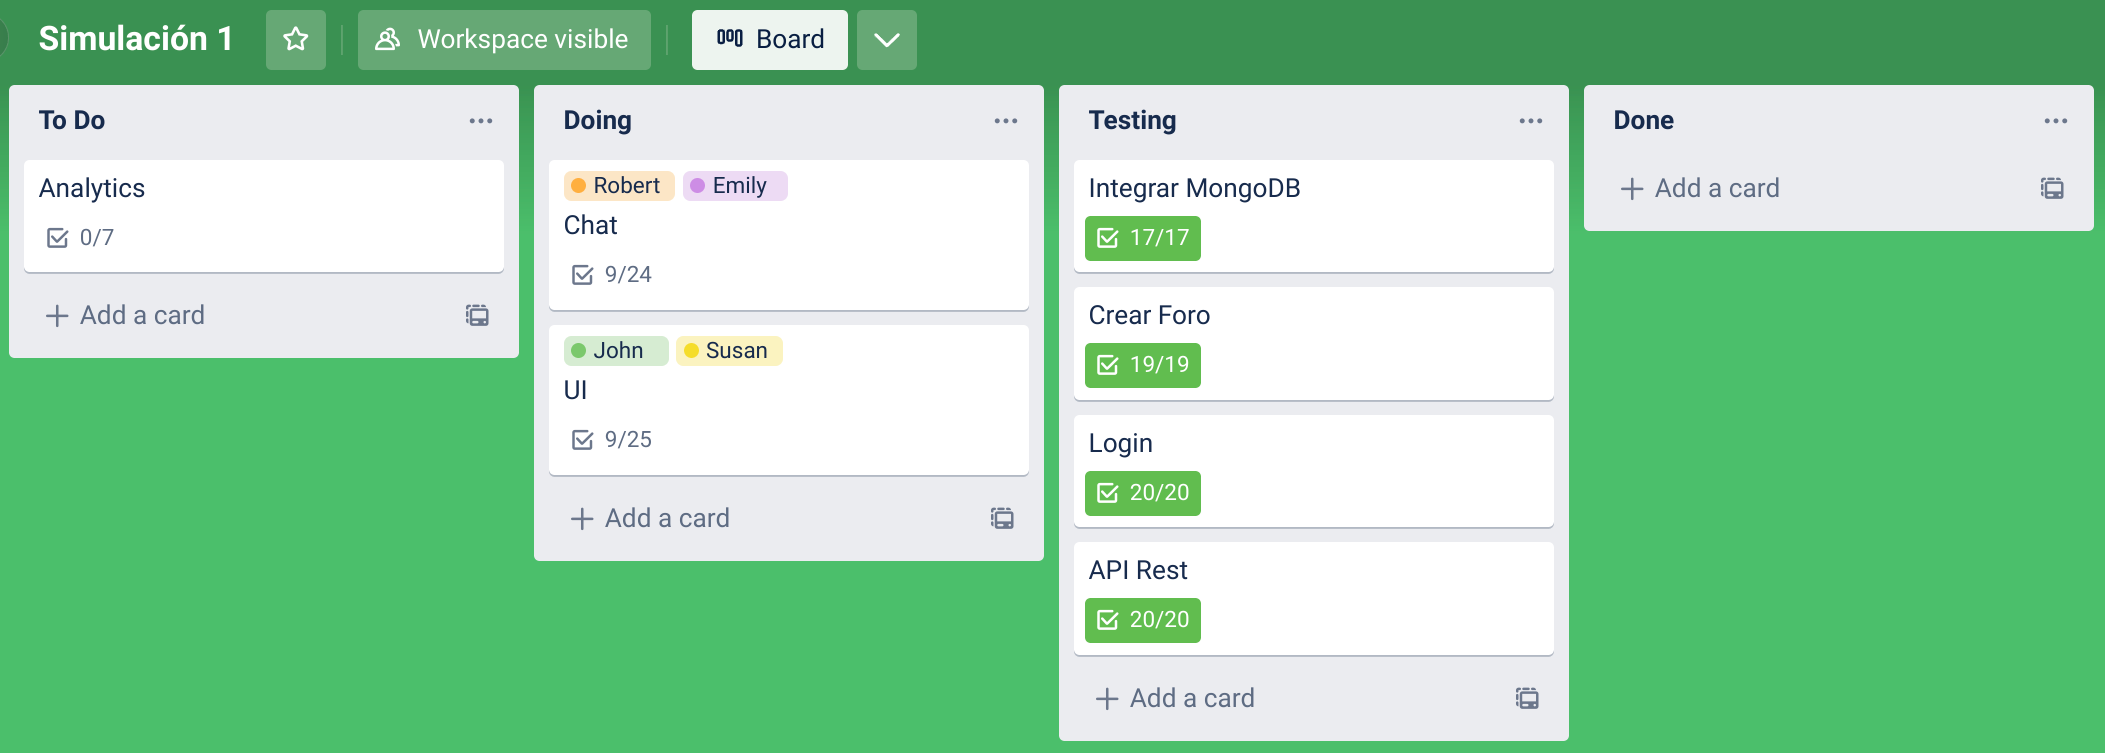
\includegraphics[width=\linewidth]{img/s1-7.png}
\end{center}

\subsection{Reunión 8}
Teniendo en cuenta el estado de las tareas, no es posible que hoy se termine ninguna. También el equipo se da cuenta que la estimación de la tarea “Chat” no ha sido adecuada, porque se van a necesitar más días.

\begin{columntblr}{XX[2]XXX}
    Reunión 8 & Tarea actual & Avance diario & Estado final/día & Días usados\\
    John & UI & 2 & 14/25 & 3/5\\
    Susan & UI & 3 & 14/25 & 3/5\\
    Emily & Chat & 1 & 16/24 & 4/4\\
    Robert & Chat & 6 & 16/24 & 4/4\\
\end{columntblr}

\begin{center}
    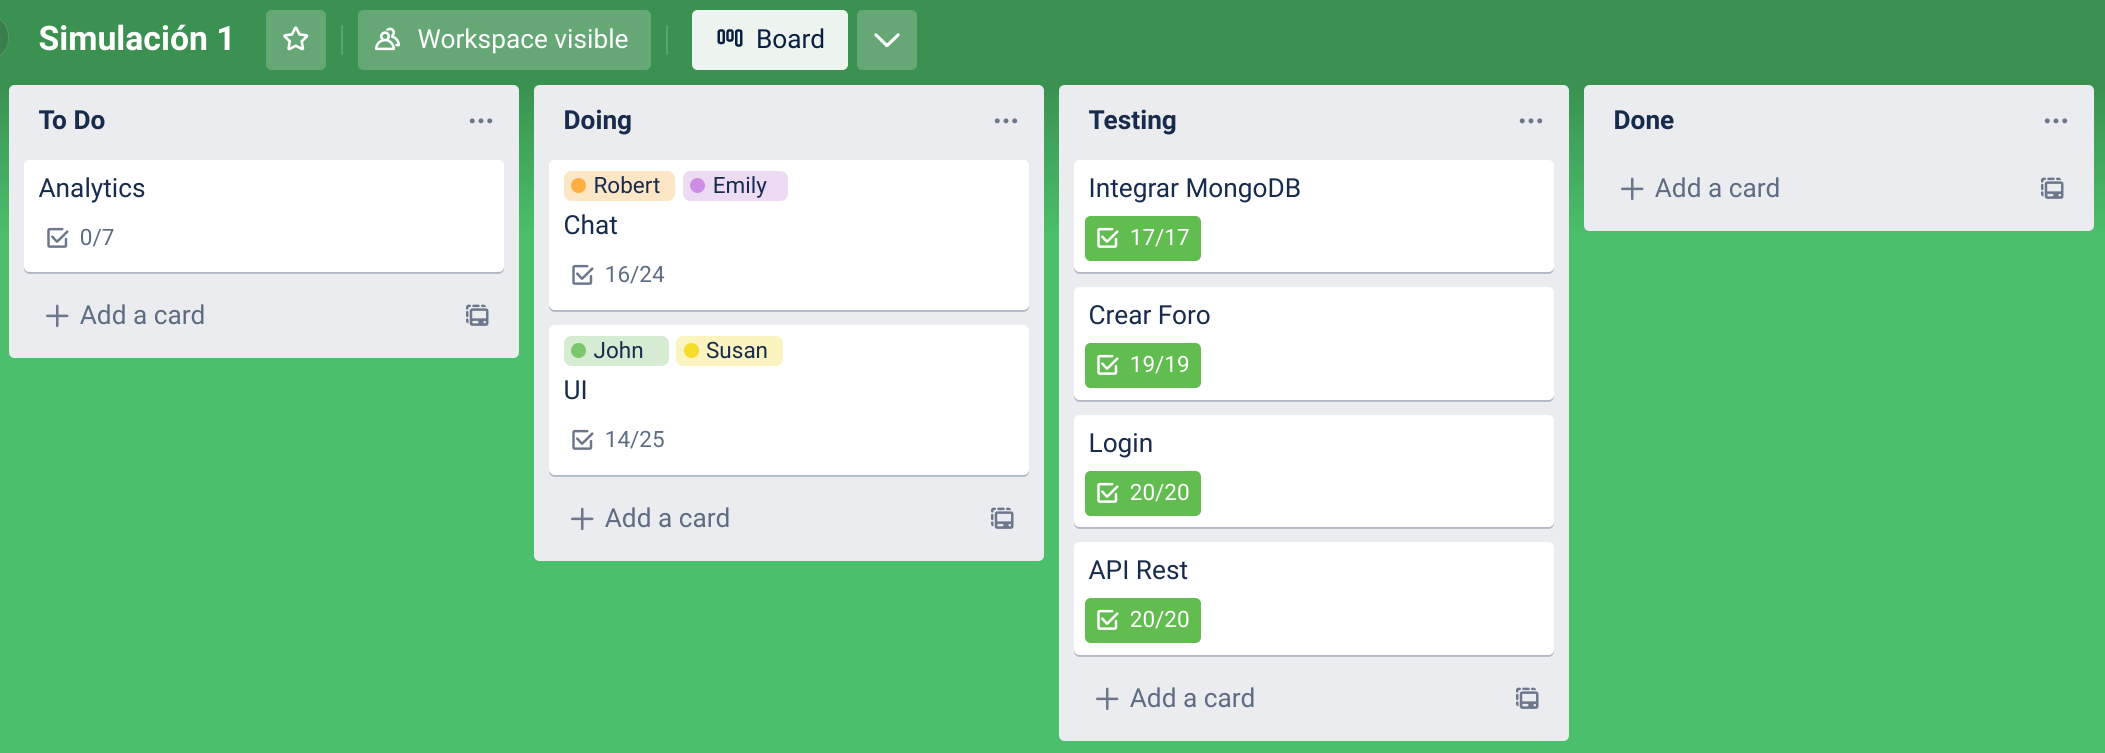
\includegraphics[width=\linewidth]{img/s1-8.png}
\end{center}

\subsection{Reunión 9}
Tal como se supuso en la reunión de ayer, la tarea “Chat” va a requerir más tiempo. Se estima que hoy se terminará la tarea “Chat”. En caso de ser así, el primero en terminar se le asignará la tarea “Analytics” y el resto del equipo cogerá una tarea para testear en la que no haya participado.

\begin{columntblr}{XX[2]XXX}
    Reunión 9 & Tarea actual & Avance diario & Estado final/día & Días usados\\
    John & UI & 5 & 20/25 & 4/5\\
    Susan & UI & 1 & 20/25 & 4/5\\
    Emily & Chat & 2 & 23/24 & 5/4\\
    Robert & Chat & 5 & 23/24 & 5/4\\
\end{columntblr}

\begin{center}
    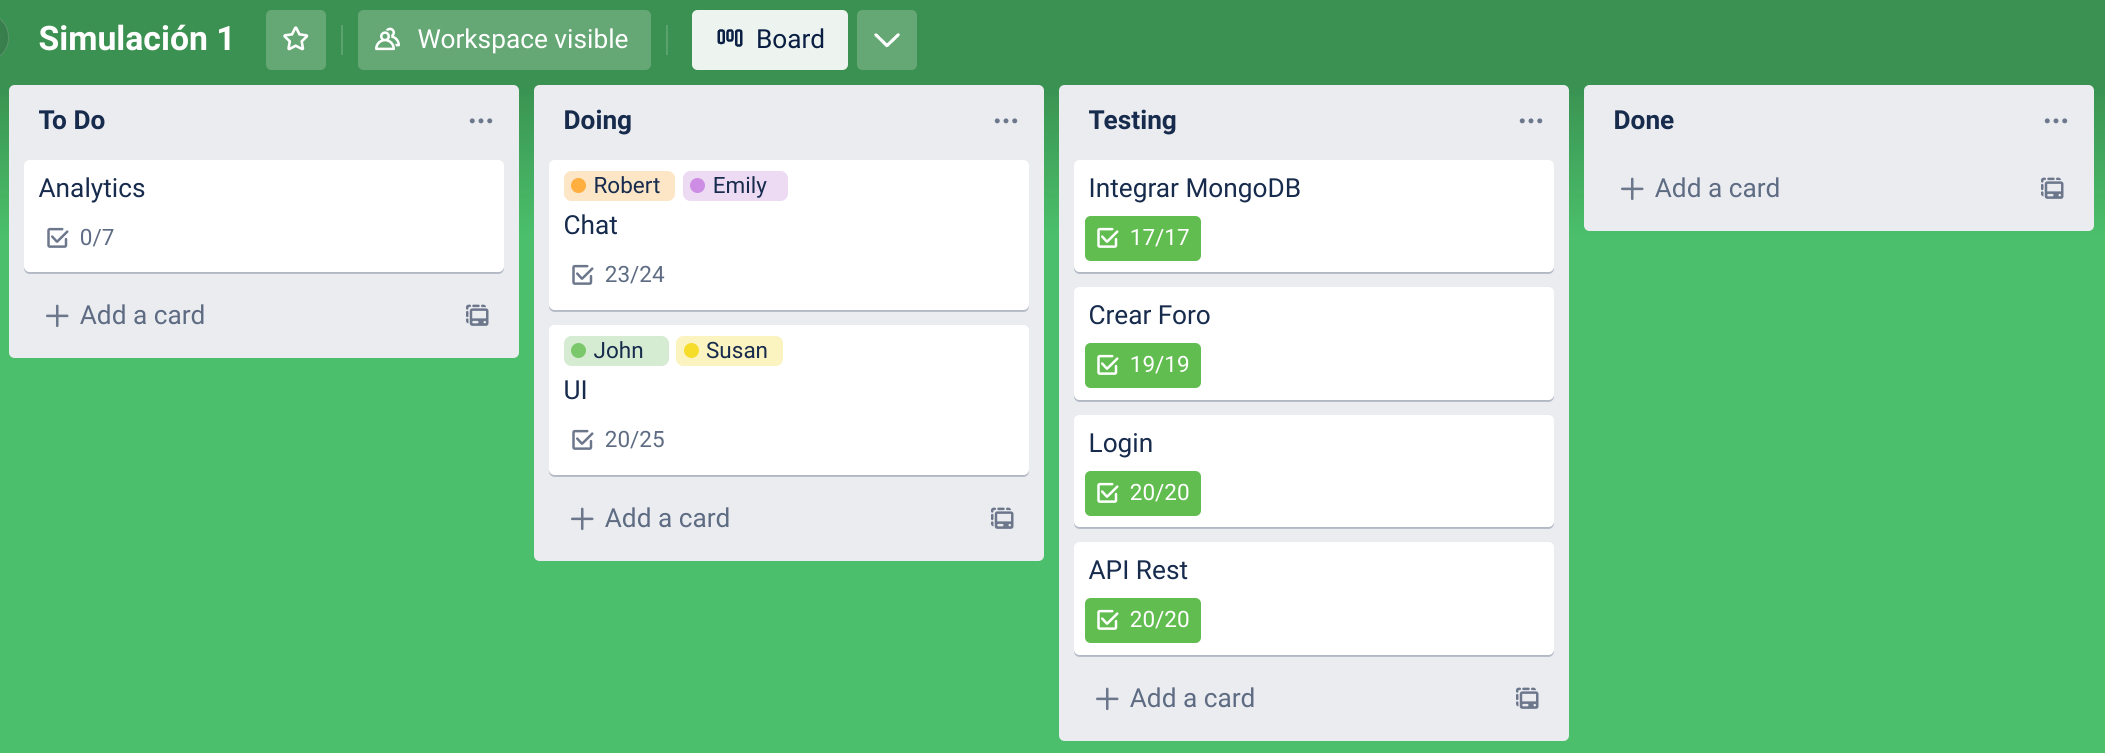
\includegraphics[width=\linewidth]{img/s1-9.png}
\end{center}

\subsection{Reunión 10}
Teniendo en cuenta el avance de ayer, se decide que John y Susan sigan con la tarea UI hasta que la terminen, y cuando terminen uno coja “Analytics” y si eso la otra persona coja una tarea para testear.

Al final la estimación de “Chat” de ayer no fue correcta, pero está a punto de terminarse. Se decide que la termine Emily en solitario y Robert se ponga a testear “Login”.

Dado que para la fase de “Testing” no se ha estimado tiempo, se decide que se utilice lo que quede de día para dicha labor.

\begin{columntblr}[long]{XX[2]XXX}
    Reunión 10 & Tarea actual & Avance diario & Estado final/día & Días usados\\
    John & UI & 3 & 25/25 & 5/5\\
    Susan & UI & 2 & 25/25 & 5/5\\
    Emily & Chat & 1 & 24/24 & 6/4\\
    Robert & Test-Login &  &  & \\
    Susan & Analytics & 4 & 4/7 & 1/4\\
    Emily & Test-API Rest &  & & \\
\end{columntblr}

\begin{center}
    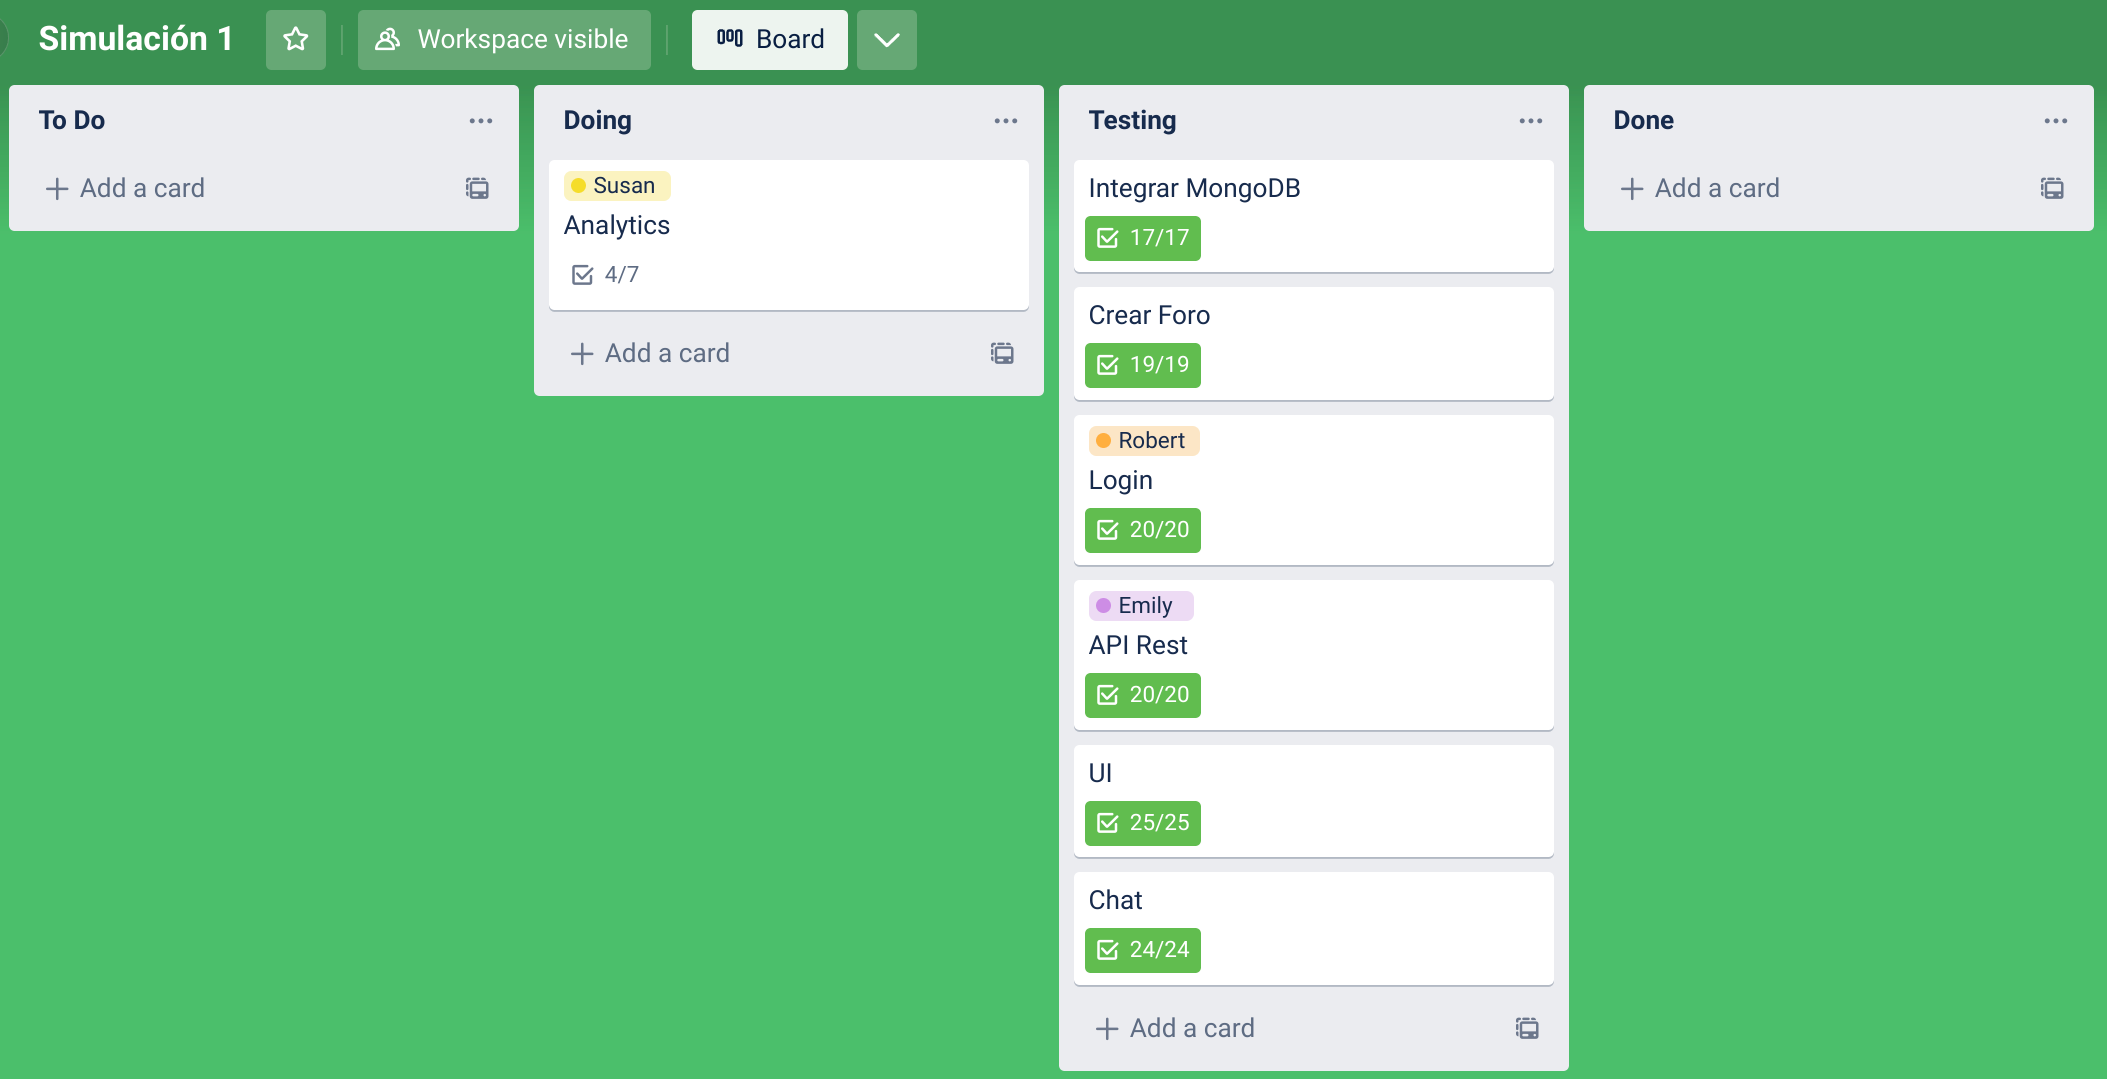
\includegraphics[width=\linewidth]{img/s1-10.png}
\end{center}


\subsection{Reunión 11}
Dado que ayer John y Susan terminaron su tarea, pero John no tuvo tiempo de hacer nada más, hoy se dedica a testear 2 tareas que no ha realizado (“Integrar MongoDB” y “Crear Foro”). Susan tratará de terminar “Analytics”, y de terminar, pasará a fase de testeo de “Chat”.

Por otro lado, Robert y Emily terminarán de testear las tareas y ambos pasarán a testear UI.

\begin{columntblr}[long]{XX[2]XXX}
    Reunión 11 & Tarea actual & Avance diario & Estado final/día & Días usados\\
    John & Test {MongoDB y Foro} &  &  & \\
    Susan & Analytics & 3 & 7/7 & 2/4\\
    Susan & Test-Chat & & &\\
    Robert & Test-UI &  &  & \\
    Emily & Test-UI &  & & \\
\end{columntblr}

\begin{center}
    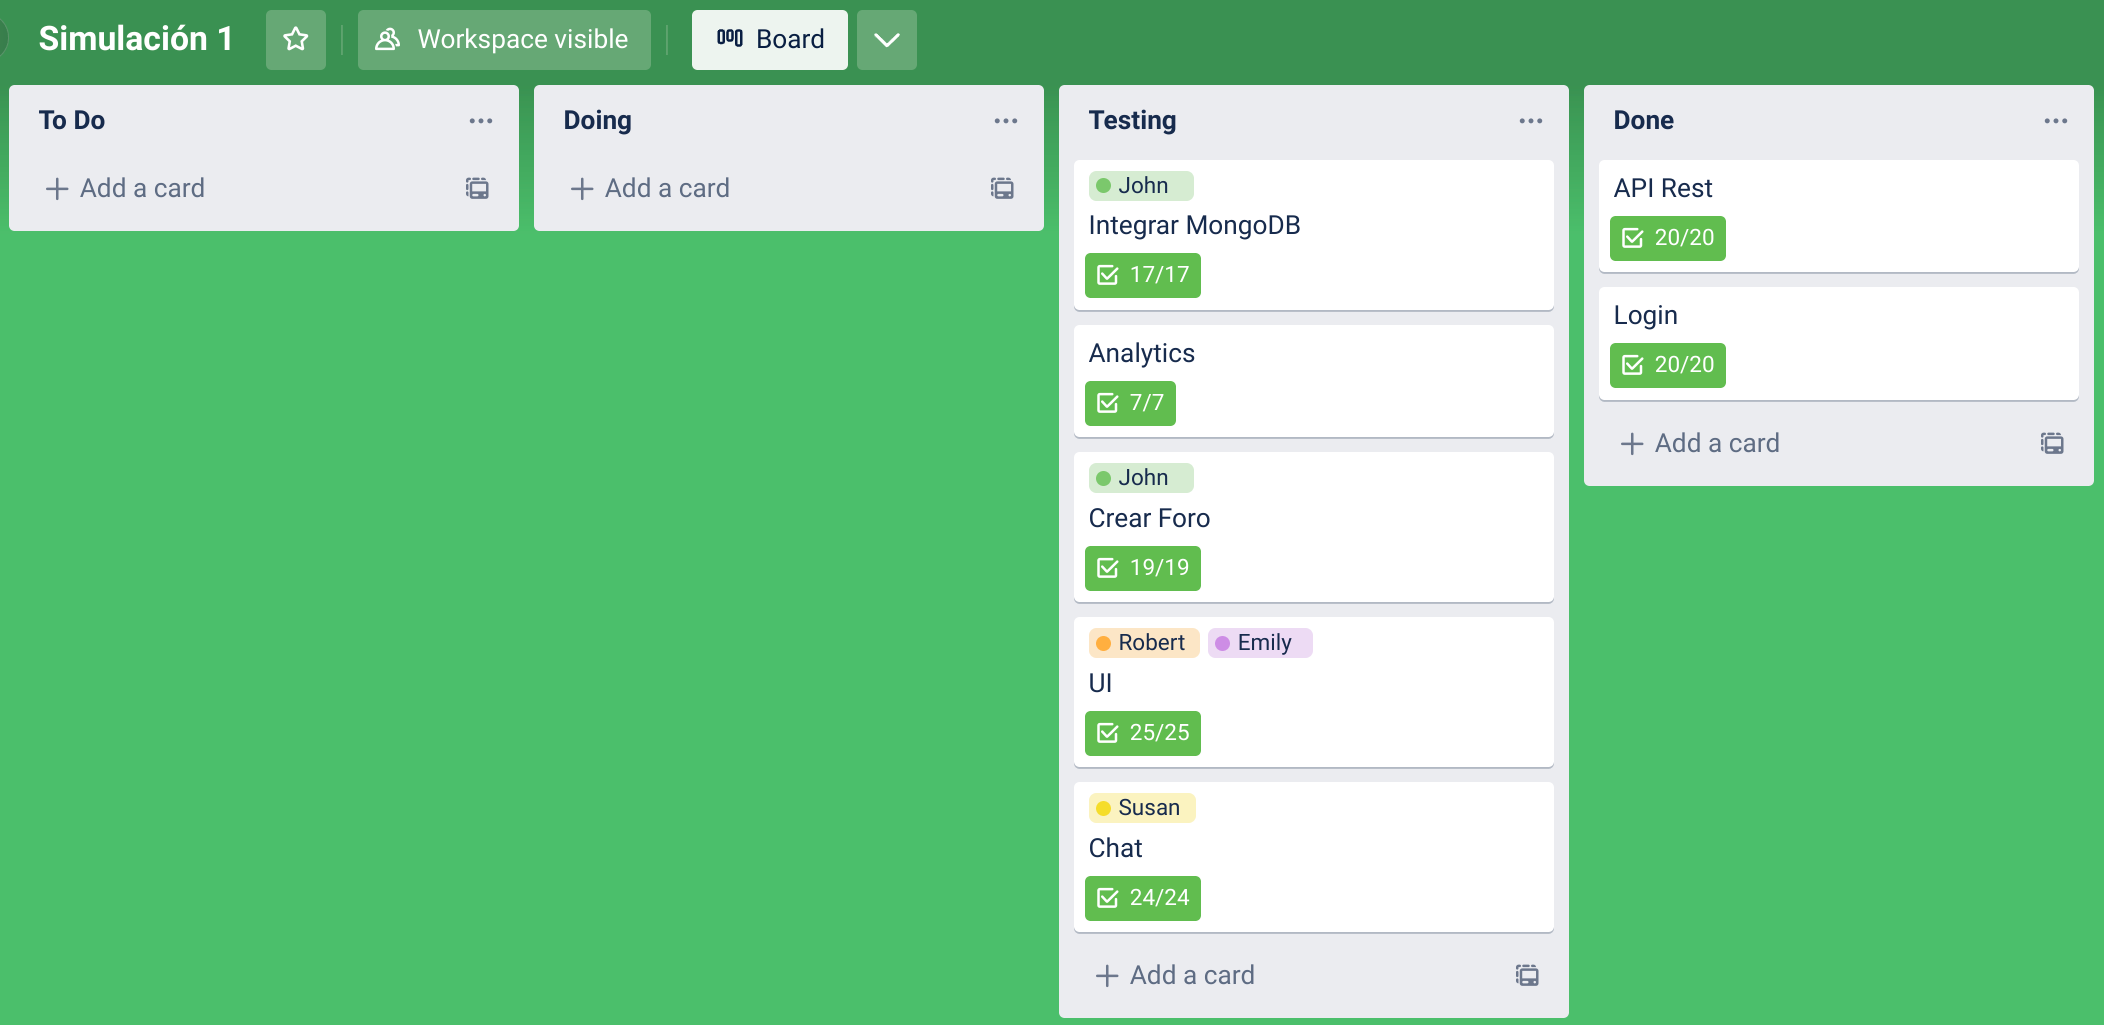
\includegraphics[width=\linewidth]{img/s1-11.png}
\end{center}

\subsection{Reunión 12}
Con los avances realizados ayer, la única tarea que queda por testear es “Analytics”, que será asignada a Robert.

Entre todo el equipo se decide que, salvo sorpresa, el proyecto termina el día de hoy, ya que no hay más tareas para realizar ni testear.

\begin{columntblr}[long]{XXXXX}
    Reunión 12 & Tarea actual & Avance diario & Estado final/día & Días usados\\
    Robert & Test-Analytics &  &  & \\
\end{columntblr}

\begin{center}
    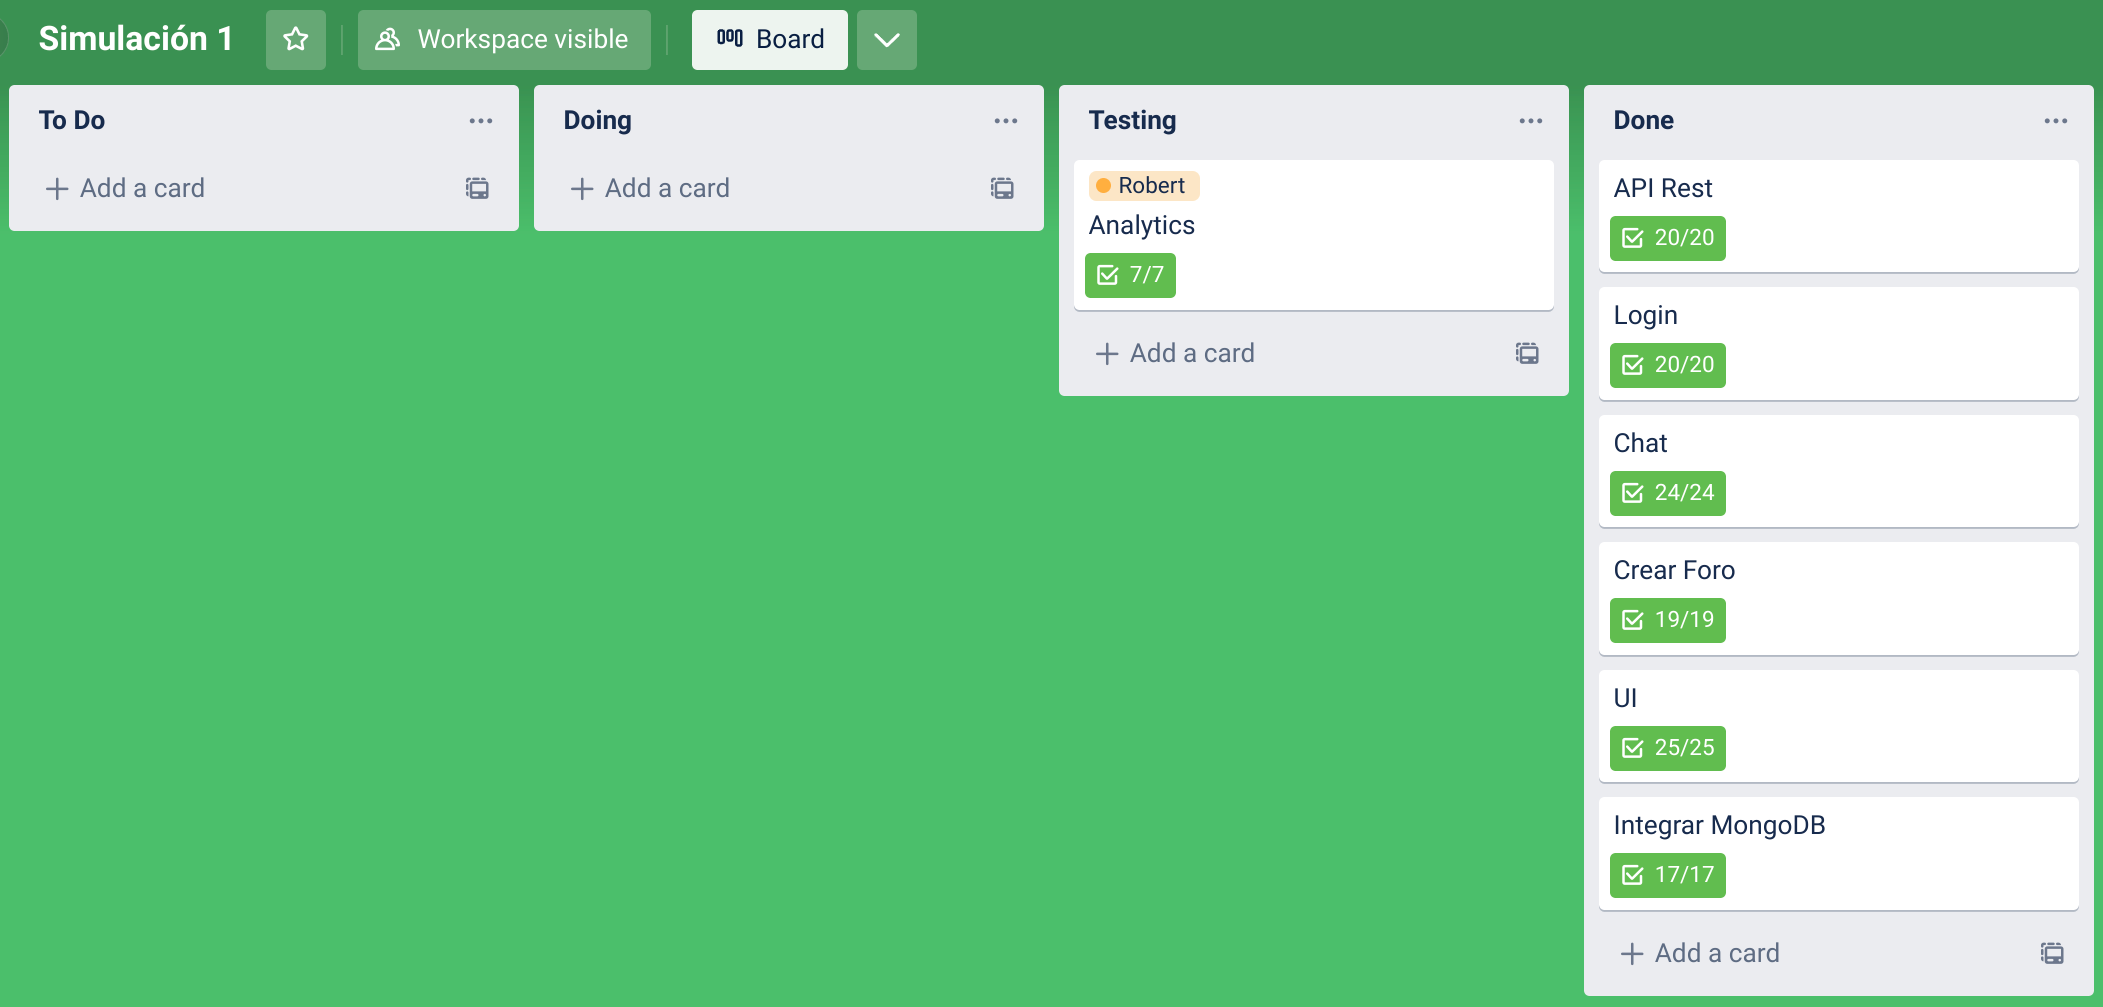
\includegraphics[width=\linewidth]{img/s1-12.png}
\end{center}

\subsection{Resumen de la Simulación 1}
A continuación se va a detallar el resumen de lo acontecido durante la simulación:

\textbf{¿La estimación temporal fue la correcta?}
\begin{itemize}
    \item La estimación inicial de ciertas tareas no ha sido del todo correcta. Para tareas cortas como “Analytics” se ha estimado 4 días y para otras más largas como “Chat”, de 24 horas, el mismo número de días.

    Por otro lado, y si seguimos comparando “Chat”, para otras tareas con menos horas (“Login” y “API Rest”) se les ha otorgado más días.

    Se puede decir que ha habido poco consenso en la estimación de días si se realiza la comparación entre tareas.
\end{itemize}

\textbf{¿Qué hubierais cambiado del planteamiento inicial? ¿Qué factores hubierais tenido en cuenta?}

\begin{itemize}
    \item El cambio principal sería la modificación de la estimación inicial de días. Se podría haber establecido que la necesidad de días fuese el número de horas entre 4. Por lo tanto, quedaría algo similar a lo siguiente (se han redondeado algunos resultados):

    \begin{columntblr}[long]{XXX}
        Tareas de programación & Coste & Límite inicial
        establecido (días) \\
        Login & 20 & 5 \\
        API Rest & 20 & 5 \\
        Integrar MongoDB & 17 & 4 \\
        Crear Foro & 19 & 5 \\
        UI & 25 & 6 \\
        Chat & 24 & 6 \\
        Analytics & 7 & 2 \\
    \end{columntblr}
\end{itemize}

\textbf{¿Cuántas veces durante el proceso se han cambiado las fechas límites?}

\begin{itemize}
    \item Se han tenido que hacer tres cambios a lo largo del proyecto, aunque dos de los cambios han sido para la estimación de la misma tarea (“Chat”, que al final ha requerido de 6 días aunque habían sido estimados 4).
\end{itemize}


\textbf{¿Se han ajustado bien los nuevos plazos establecidos o han sobrado recursos tras los reajustes?}

\begin{itemize}
    \item Aunque en los reajustes ha sobrado tiempo, acto seguido se ha puesto con la nueva tarea a realizar. De esta manera se ha aprovechado de manera correcta el tiempo.
\end{itemize}


\textbf{¿Cómo habéis consensuado las decisiones para reajustar los recursos?}

\begin{itemize}
    \item Teniendo en cuenta el planteamiento anterior propuesto de estimar que van a ser “4 horas/día”. En el caso de “Chat”, faltaban 8 horas y había dos personas realizando la tarea, por eso en primera instancia se decidió que con un día más habría sido suficiente.

    Al final no fue así, y por tanto se necesitó de un día más de una persona, ya que a la otra se le asignó a otra tarea.
\end{itemize}

\textbf{¿Qué nuevas decisiones propondríais para futuros proyectos?}
\begin{itemize}
    \item Aparte de la proposición comentada previamente para la estimación de días, se cree que es necesario realizar un nuevo añadido a las estimaciones.

    Esta nueva estimación sería la de el tiempo que se va a requerir para realizar la fase de testeo de las actividades. Se podría indicar que el tiempo de testeo puede ser el de el número de horas de desarrollo entre 6, aunque lógicamente cada caso puede tarea puede ser distinta.
\end{itemize}



\chapter{Conclusiones}

Tal como se ha podido ver a lo largo del documento,

\end{document}
